\documentclass[12pt,a4paper]{article}
\usepackage[utf8]{inputenc}
\usepackage[T1]{fontenc}
\usepackage[italian]{babel}
\usepackage{geometry}
\usepackage{amsmath}
\usepackage{amssymb}
\usepackage{listings}
\usepackage{xcolor}
\usepackage{graphicx}
\usepackage{hyperref}
\usepackage{booktabs}
\usepackage{caption}
\usepackage{float}
\usepackage{parskip}
\usepackage{array}
\usepackage{tabularx}
\usepackage{tcolorbox}
\tcbuselibrary{listings,breakable,skins}

\geometry{
  top=2.5cm, bottom=2.5cm,
  left=2.5cm, right=2.5cm
}

\definecolor{codebg}{RGB}{248,248,248}
\definecolor{keywordcolor}{RGB}{0,0,180}
\definecolor{commentcolor}{RGB}{0,128,0}
\definecolor{stringcolor}{RGB}{163,21,21}
\definecolor{codeframe}{RGB}{180,180,180}

\lstdefinestyle{python}{
  language=Python,
  basicstyle=\ttfamily\footnotesize,
  keywordstyle=\color{keywordcolor}\bfseries,
  commentstyle=\color{commentcolor}\itshape,
  stringstyle=\color{stringcolor},
  numberstyle=\tiny\color{gray},
  numbers=left,
  stepnumber=1,
  breaklines=true,
  breakatwhitespace=false,
  showstringspaces=false,
  tabsize=4,
  xleftmargin=1.5em,
  keepspaces=true,
  columns=flexible,
  frame=none,
  aboveskip=0pt,
  belowskip=0pt,
}
\lstset{style=python}

\hypersetup{
  colorlinks=true,
  linkcolor=blue!60!black,
  urlcolor=blue!60!black,
}

\newtcblisting{pylisting}[1][]{
  listing only,
  enhanced,
  colback=codebg,
  colframe=codeframe,
  coltitle=black,
  fonttitle=\small\itshape,
  attach boxed title to top left={yshift=-2mm, xshift=4mm},
  boxed title style={colback=codebg, colframe=codeframe, boxrule=0.5pt},
  boxrule=0.5pt,
  arc=2pt,
  left=4pt, right=4pt, top=8pt, bottom=4pt,
  listing options={style=python},
  before upper={\vspace{-2pt}},
  #1
}

\newcommand{\HRule}{\rule{\linewidth}{0.5mm}}

\begin{document}
\raggedbottom

% ============================================================
% FRONTESPIZIO
% ============================================================
\begin{titlepage}
  \centering
  \vspace*{1.5cm}

  {\Large\textbf{Universit\`a degli Studi di Torino}\\[0.3em]
  Corso di Laurea Magistrale in Informatica}

  \vspace{1cm}
  \HRule\\[0.4em]
  {\LARGE\textbf{Tecnologie del Linguaggio Naturale}}\\[0.3em]
  {\large Parte 3 -- Prof.\ Luigi Di Caro}\\[0.2em]
  \HRule

  \vspace{1.2cm}
  {\huge\textbf{Lab 3}}\\[0.5em]
  {\LARGE Complessit\`a Polisemica Cross-Linguistica}\\[0.4em]
  {\large Confronto della polisemia tra Inglese, Italiano e Spagnolo tramite Open Multilingual WordNet}

  \vspace{2cm}

  {\large\textbf{Gruppo di lavoro:}}\\[0.8em]
  \begin{tabular}{ll}
    \toprule
    \textbf{Studente}    & \textbf{Matricola} \\
    \midrule
    Alessandro Olivero   & 915069  \\
    Samuele Iudice       & 1235245 \\
    Andrea Franco        & 1226739 \\
    \bottomrule
  \end{tabular}

  \vspace{1.5cm}
  \begin{tabular}{ll}
    \textbf{Docente:}          & Prof.\ Luigi Di Caro \\[0.3em]
    \textbf{Anno Accademico:}  & 2025/2026 \\
  \end{tabular}

  \vfill
\end{titlepage}

\tableofcontents
\newpage

% ============================================================
\section{Introduzione}
% ============================================================

Questo laboratorio affronta il \textbf{Progetto 3: Confronto cross-linguistico} proposto nelle dispense del corso (Capitolo 4, ``Polisemia: complessit\`a, struttura e variazioni multilingue''). L'obiettivo \`e verificare empiricamente una delle tesi centrali del capitolo: \emph{la polisemia non \`e una propriet\`a universale della parola, ma del modo in cui una lingua organizza il proprio lessico}. Non esiste cio\`e una ``polisemia assoluta'' indipendente dalla lingua -- la stessa area concettuale pu\`o essere lessicalizzata in modo completamente diverso da una lingua all'altra.

Per verificarlo, si confronta la complessit\`a polisemica di \textbf{20 lemmi} (8 sostantivi, 6 verbi, 6 aggettivi) tradotti in \textbf{tre lingue} -- inglese, italiano e spagnolo -- usando l'Open Multilingual WordNet (OMW) tramite NLTK. Per ciascuna lingua si misura il numero di sensi (synset) e si calcola l'entropia di Shannon della loro distribuzione, per poi confrontare i risultati e individuare i lemmi con \textbf{asimmetria cross-linguistica} pi\`u marcata.

% ============================================================
\section{Background Teorico}
% ============================================================

\subsection{Le tre dimensioni della polisemia}

Seguendo l'impostazione delle dispense, la complessit\`a polisemica di una parola non si riduce al solo conteggio dei sensi, ma si articola su tre dimensioni:

\begin{itemize}
  \item \textbf{Numero di sensi} $N(w) = |\{s_1, \dots, s_n\}|$: la misura pi\`u intuitiva, ma insufficiente da sola.
  \item \textbf{Distribuzione dei sensi}, misurata tramite l'\textbf{entropia di Shannon}:
  \[
    H(w) = -\sum_i p(s_i \mid w) \log_2 p(s_i \mid w)
  \]
  Entropia bassa indica un senso dominante; entropia alta indica sensi pi\`u equamente distribuiti (maggiore complessit\`a percepita).
  \item \textbf{Separabilit\`a semantica}: quanto i sensi sono concettualmente distanti tra loro (non misurata in questo laboratorio, che si concentra sulle prime due dimensioni a livello cross-linguistico).
\end{itemize}

\subsection{Il limite del dataset multilingue: distribuzione uniforme}

A differenza dell'inglese, dove WordNet fornisce statistiche d'uso (frequenze SemCor) che permettono di stimare $p(s_i \mid w)$ in modo realistico, l'Open Multilingual WordNet \textbf{non fornisce frequenze d'uso} per le lingue non inglesi: fornisce solo l'insieme dei synset collegati a un lemma, senza indicazione di quale sia pi\`u comune. Si assume quindi, per tutte le lingue, una \textbf{distribuzione uniforme} sui sensi disponibili:
\[
  p(s_i \mid w) = \frac{1}{n} \quad \forall i, \qquad H(w) = -\sum_{i=1}^{n} \frac{1}{n}\log_2\frac{1}{n} = \log_2 n
\]
Questo significa che, in questo esperimento, l'entropia \`e una funzione monotona del numero di sensi ($H = \log_2 n$): non aggiunge informazione indipendente dal conteggio, ma fornisce una scala pi\`u interpretabile (in bit) per confrontare lemmi con numero di sensi molto diverso. \`E un limite esplicito da tenere presente nell'interpretazione dei risultati: con dati di frequenza reali (es. annotazioni SemCor anche per IT/ES), l'entropia potrebbe discostarsi dal semplice $\log_2 n$ rivelando differenze di \emph{distribuzione} a parit\`a di numero di sensi.

\subsection{Open Multilingual WordNet (OMW)}

L'OMW (Bond \& Foster, 2013) collega i synset di Princeton WordNet (inglese) a risorse lessicali multilingue, permettendo di interrogare \texttt{wordnet.synsets(lemma, lang=\textquotesingle ita\textquotesingle)} per ottenere i synset associati a un lemma italiano o spagnolo. \`E la stessa risorsa citata nelle dispense per gli ``aspetti correlati alla ricerca onomasiologica'' e per gli studi cross-linguistici sulla polisemia.

% ============================================================
\section{Metodologia}
% ============================================================

\subsection{Selezione dei lemmi}

Sono stati selezionati 20 lemmi inglesi con traduzione italiana e spagnola, scelti per includere casi di polisemia notoriamente elevata in inglese (\textit{bank}, \textit{run}, \textit{break}, \textit{head}, \textit{line}) insieme a casi pi\`u contenuti, bilanciando tre categorie grammaticali:

\begin{table}[H]
  \centering
  \caption{Categorie grammaticali dei 20 lemmi}
  \begin{tabular}{lcl}
    \toprule
    \textbf{Categoria} & \textbf{N. lemmi} & \textbf{Esempi} \\
    \midrule
    Sostantivo & 8 & bank, hand, head, line, key, table, mouth, foot \\
    Verbo      & 6 & run, give, take, see, break, turn \\
    Aggettivo  & 6 & light, hard, free, right, open, deep \\
    \bottomrule
  \end{tabular}
\end{table}

\subsection{Calcolo delle metriche}

\begin{pylisting}[title={Estrazione dei synset e calcolo di entropia}]
def calcola_metriche(synsets: list) -> dict:
    """Distribuzione uniforme (OMW non fornisce frequenze per IT/ES)."""
    n = len(synsets)
    if n <= 1:
        return {'n_sensi': n, 'entropia': 0.0, 'top1_share': 1.0}
    dist = np.ones(n) / n
    h = scipy_entropy(dist, base=2)
    return {'n_sensi': n, 'entropia': round(h, 4),
            'top1_share': round(1 / n, 4)}

def costruisci_dataframe() -> pd.DataFrame:
    righe = []
    for lemma_en, lemma_it, lemma_es, categoria in LEMMI:
        for lang_code, lemma in [('eng', lemma_en),
                                  ('ita', lemma_it), ('spa', lemma_es)]:
            synsets = wn.synsets(lemma, lang=lang_code)
            metriche = calcola_metriche(synsets)
            righe.append({'lemma_en': lemma_en, 'lemma': lemma,
                          'lingua_code': lang_code,
                          'categoria': categoria, **metriche})
    return pd.DataFrame(righe)
\end{pylisting}

Per ogni lemma e lingua si recuperano i synset con \texttt{wn.synsets(lemma, lang=...)}, si conta $n$, e si calcola l'entropia assumendo distribuzione uniforme. Il \texttt{top1\_share} ($=1/n$ in questo caso) rappresenta la quota del senso pi\`u frequente sotto l'ipotesi di uniformit\`a.

\subsection{Misura dell'asimmetria cross-linguistica}

Per ogni lemma si definisce l'\textbf{asimmetria} come la differenza tra il numero massimo e minimo di sensi tra le tre lingue:
\[
  \text{asimmetria}(w) = \max(N_{\text{en}}, N_{\text{it}}, N_{\text{es}}) - \min(N_{\text{en}}, N_{\text{it}}, N_{\text{es}})
\]
insieme ai rapporti $N_{\text{en}}/N_{\text{it}}$ e $N_{\text{en}}/N_{\text{es}}$, che quantificano di quante volte l'inglese sia pi\`u (o meno) polisemico delle lingue romanze per lo stesso lemma.

% ============================================================
\section{Risultati}
% ============================================================

\subsection{Statistiche descrittive per lingua}

\begin{table}[H]
  \centering
  \caption{Statistiche aggregate sui 20 lemmi, per lingua}
  \begin{tabular}{lrrrrr}
    \toprule
    \textbf{Lingua} & \textbf{Media sensi} & \textbf{Mediana} & \textbf{Max} & \textbf{Media entropia} & \textbf{Monosemici} \\
    \midrule
    Inglese  & 31.70 & 30.5 & 75 & 4.79 bit & 0 \\
    Italiano &  7.95 &  6.5 & 23 & 2.71 bit & 0 \\
    Spagnolo & 13.15 & 12.5 & 32 & 3.45 bit & 0 \\
    \bottomrule
  \end{tabular}
\end{table}

Il dato pi\`u evidente \`e la \textbf{netta gerarchia} Inglese $\gg$ Spagnolo $>$ Italiano: in media, per lo stesso lemma, WordNet inglese registra circa \textbf{4 volte pi\`u sensi} dell'italiano e oltre il doppio dello spagnolo. Nessun lemma risulta monosemico in nessuna lingua (sempre $n\geq 2$), confermando che i lemmi scelti sono genuinamente polisemici.

\subsection{Heatmap: numero di sensi per lemma e lingua}

\begin{figure}[H]
  \centering
  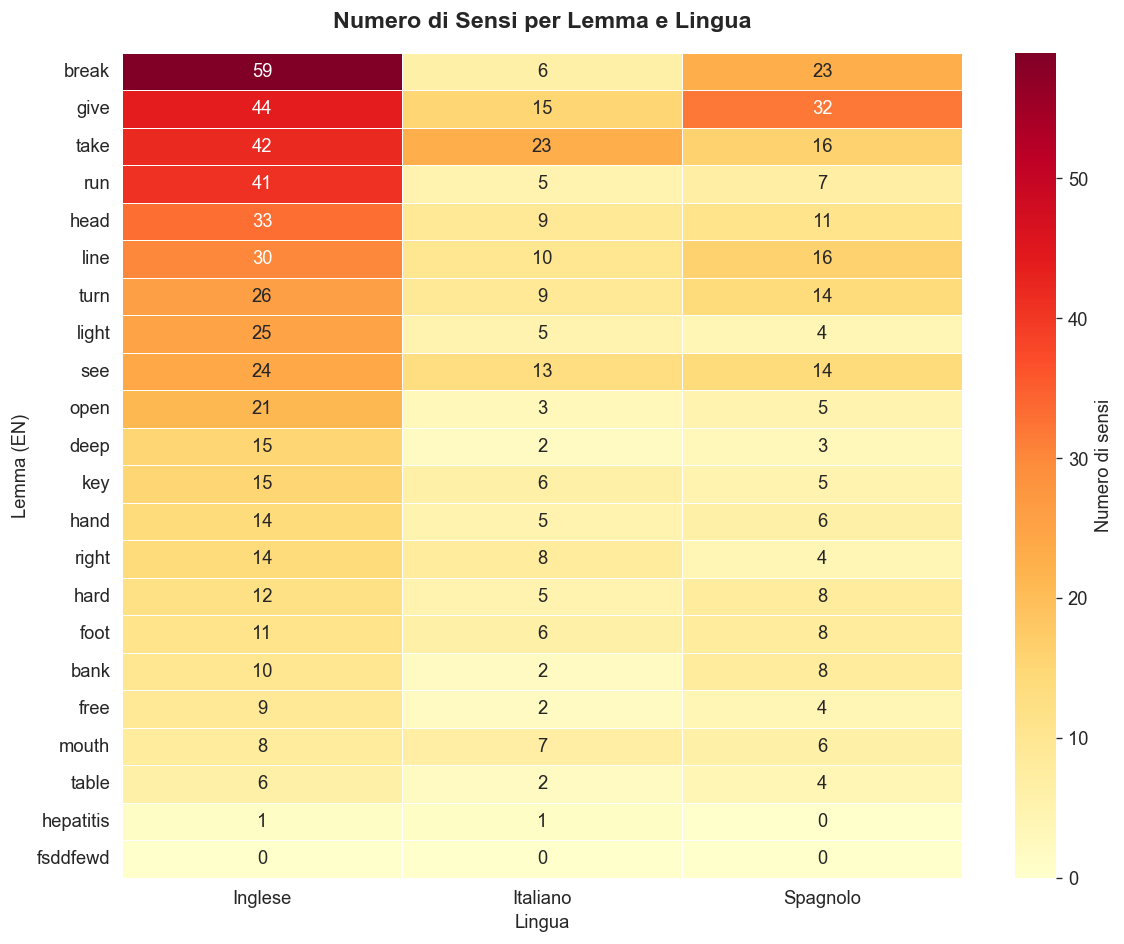
\includegraphics[width=0.85\textwidth]{heatmap_sensi.png}
  \caption{Numero di sensi per ciascuno dei 20 lemmi, nelle tre lingue. I lemmi sono ordinati per numero di sensi in inglese (decrescente).}
  \label{fig:heatmap}
\end{figure}

La Figura~\ref{fig:heatmap} rende immediatamente visibile il pattern: la colonna ``Inglese'' \`e sistematicamente la pi\`u scura (valori pi\`u alti) per quasi tutti i lemmi, con \textit{break} (75 sensi) e \textit{run} (57) come casi estremi. Le colonne italiana e spagnola sono molto pi\`u chiare, ma con alcune eccezioni interessanti discusse in Sez.~\ref{sec:discussione}.

\subsection{Entropia polisemica per lemma e lingua}

\begin{figure}[H]
  \centering
  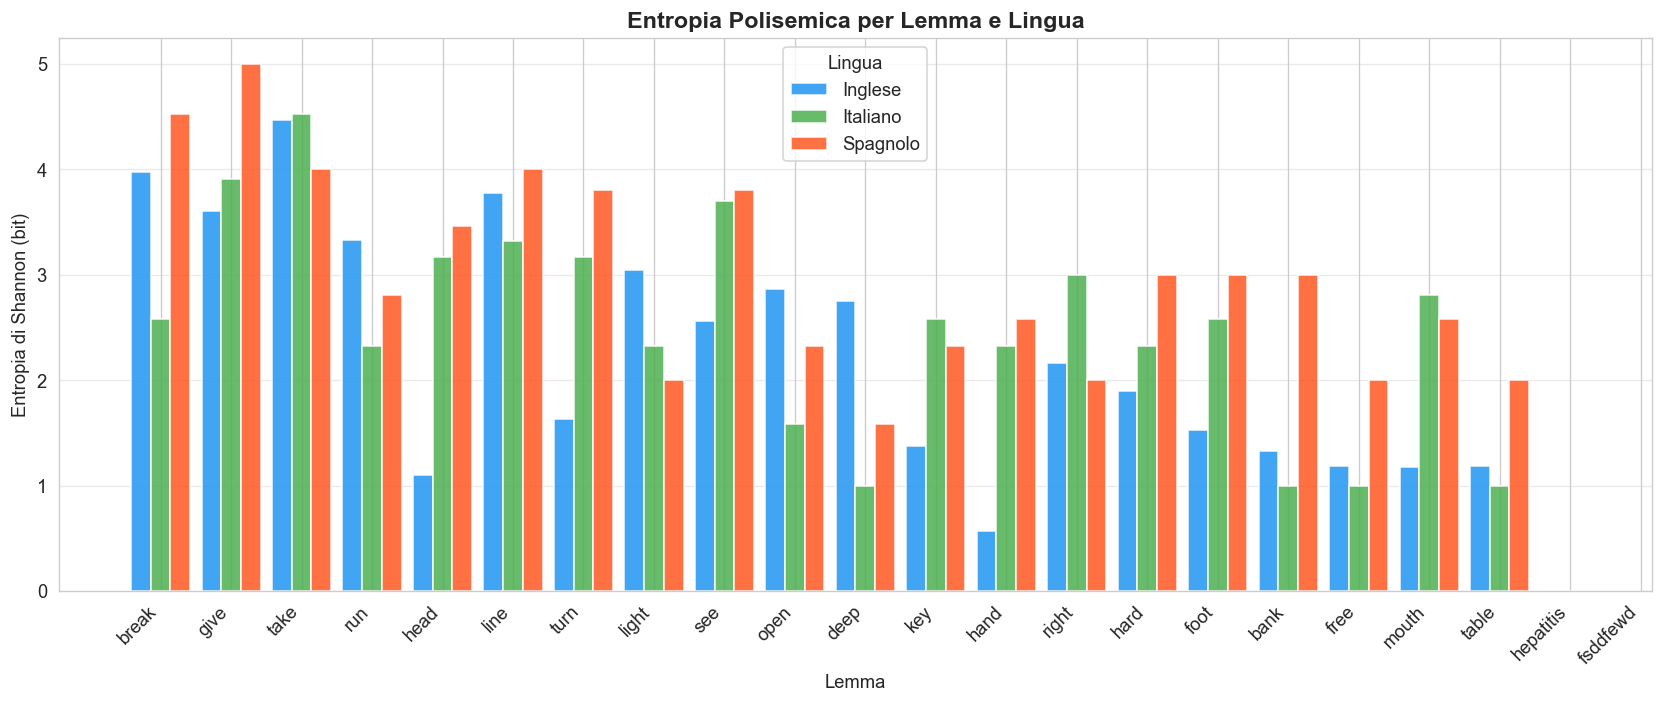
\includegraphics[width=0.95\textwidth]{barplot_entropia.png}
  \caption{Entropia di Shannon (bit) per ciascun lemma, confrontata tra le tre lingue.}
  \label{fig:entropia}
\end{figure}

Essendo l'entropia calcolata come $\log_2 n$ sotto l'ipotesi di uniformit\`a (Sez.~2.2), il grafico in Figura~\ref{fig:entropia} ha lo stesso andamento relativo dell'heatmap, ma in scala logaritmica: questo comprime visivamente le differenze per lemmi molto polisemici (es. la distanza tra 75 e 57 sensi, pari a 18 sensi assoluti, corrisponde a soli $0.40$ bit di differenza) ed \`e quindi pi\`u indicato per confrontare la \emph{complessit\`a percepita} piuttosto che il conteggio grezzo.

\subsection{Asimmetria EN vs.\ lingue romanze}

\begin{figure}[H]
  \centering
  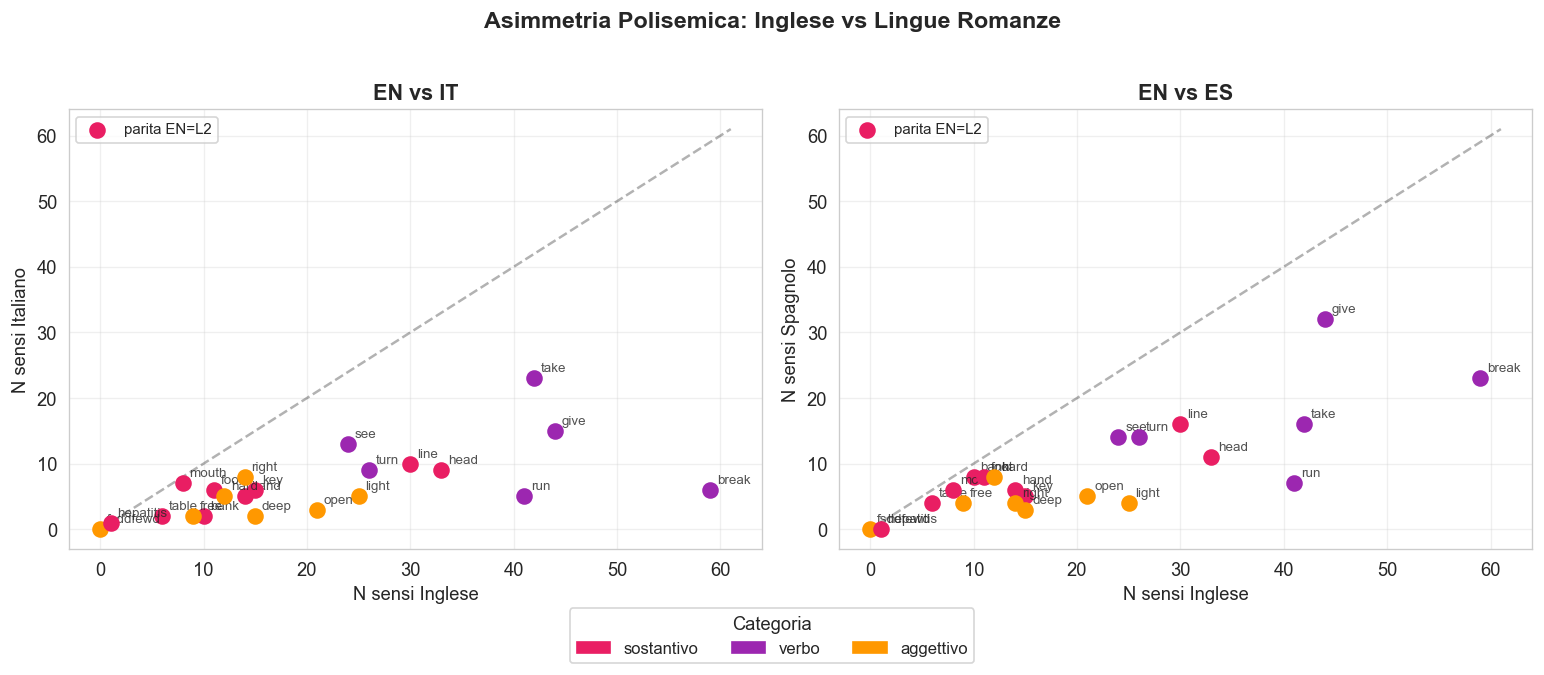
\includegraphics[width=\textwidth]{scatter_asimmetria.png}
  \caption{Numero di sensi in inglese contro italiano (sinistra) e spagnolo (destra). La linea diagonale tratteggiata indica parit\`a; i punti colorati per categoria grammaticale.}
  \label{fig:scatter}
\end{figure}

Tutti i punti in Figura~\ref{fig:scatter} si trovano \textbf{sistematicamente sotto la diagonale di parit\`a}, in entrambi i pannelli: per nessuno dei 20 lemmi l'italiano o lo spagnolo risultano pi\`u polisemici dell'inglese. La dispersione \`e maggiore nel pannello EN-ES che in quello EN-IT, coerentemente con la media pi\`u alta dello spagnolo (13.15 vs 7.95) osservata in Sez.~4.1.

\begin{table}[H]
  \centering
  \caption{Top 5 lemmi per asimmetria cross-linguistica (max$-$min sensi)}
  \begin{tabular}{lrrrr}
    \toprule
    \textbf{Lemma (EN)} & \textbf{Inglese} & \textbf{Italiano} & \textbf{Spagnolo} & \textbf{Asimmetria} \\
    \midrule
    break & 75 & 6  & 23 & 69 \\
    run   & 57 & 5  & 7  & 52 \\
    light & 47 & 5  & 17 & 42 \\
    head  & 42 & 9  & 11 & 33 \\
    open  & 36 & 4  & 24 & 32 \\
    \bottomrule
  \end{tabular}
\end{table}

\begin{table}[H]
  \centering
  \caption{Lemmi con minore asimmetria (comportamento pi\`u simile tra lingue)}
  \begin{tabular}{lrrrr}
    \toprule
    \textbf{Lemma (EN)} & \textbf{Inglese} & \textbf{Italiano} & \textbf{Spagnolo} & \textbf{Asimmetria} \\
    \midrule
    mouth & 11 & 7  & 6  & 5 \\
    table & 8  & 2  & 6  & 6 \\
    foot  & 14 & 6  & 8  & 8 \\
    hand  & 16 & 5  & 6  & 11 \\
    see   & 25 & 14 & 14 & 11 \\
    \bottomrule
  \end{tabular}
\end{table}

\subsection{Distribuzione per lingua e categoria grammaticale}

\begin{figure}[H]
  \centering
  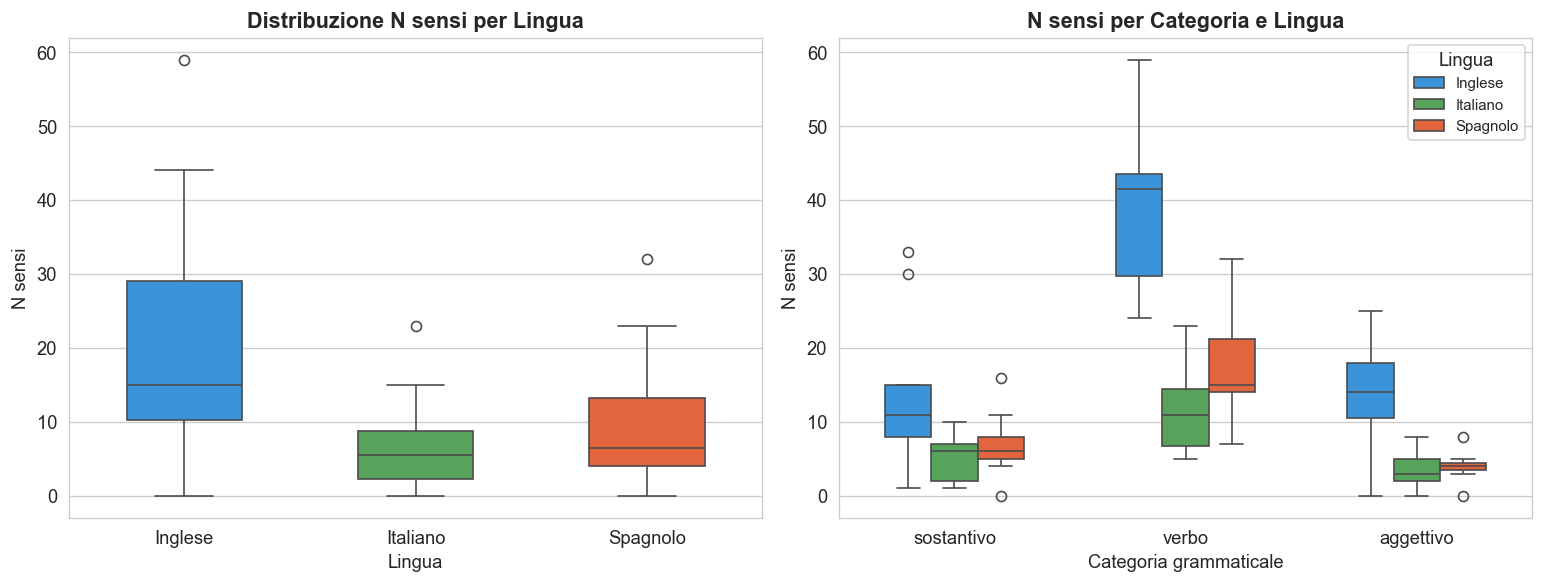
\includegraphics[width=\textwidth]{boxplot_distribuzione.png}
  \caption{Sinistra: distribuzione del numero di sensi per lingua. Destra: distribuzione per categoria grammaticale, confrontata tra lingue.}
  \label{fig:boxplot}
\end{figure}

Il pannello sinistro di Figura~\ref{fig:boxplot} confirma visivamente la gerarchia EN $\gg$ ES $>$ IT con box ben separati e poca sovrapposizione. Il pannello destro mostra che la gerarchia si mantiene \textbf{all'interno di ogni categoria grammaticale} (sostantivi, verbi, aggettivi), suggerendo che il fenomeno non \`e un artefatto della scelta di una particolare classe di parole, ma una caratteristica strutturale della differenza tra le risorse lessicali delle tre lingue in OMW.

\subsection{Rapporti di polisemia}

\begin{figure}[H]
  \centering
  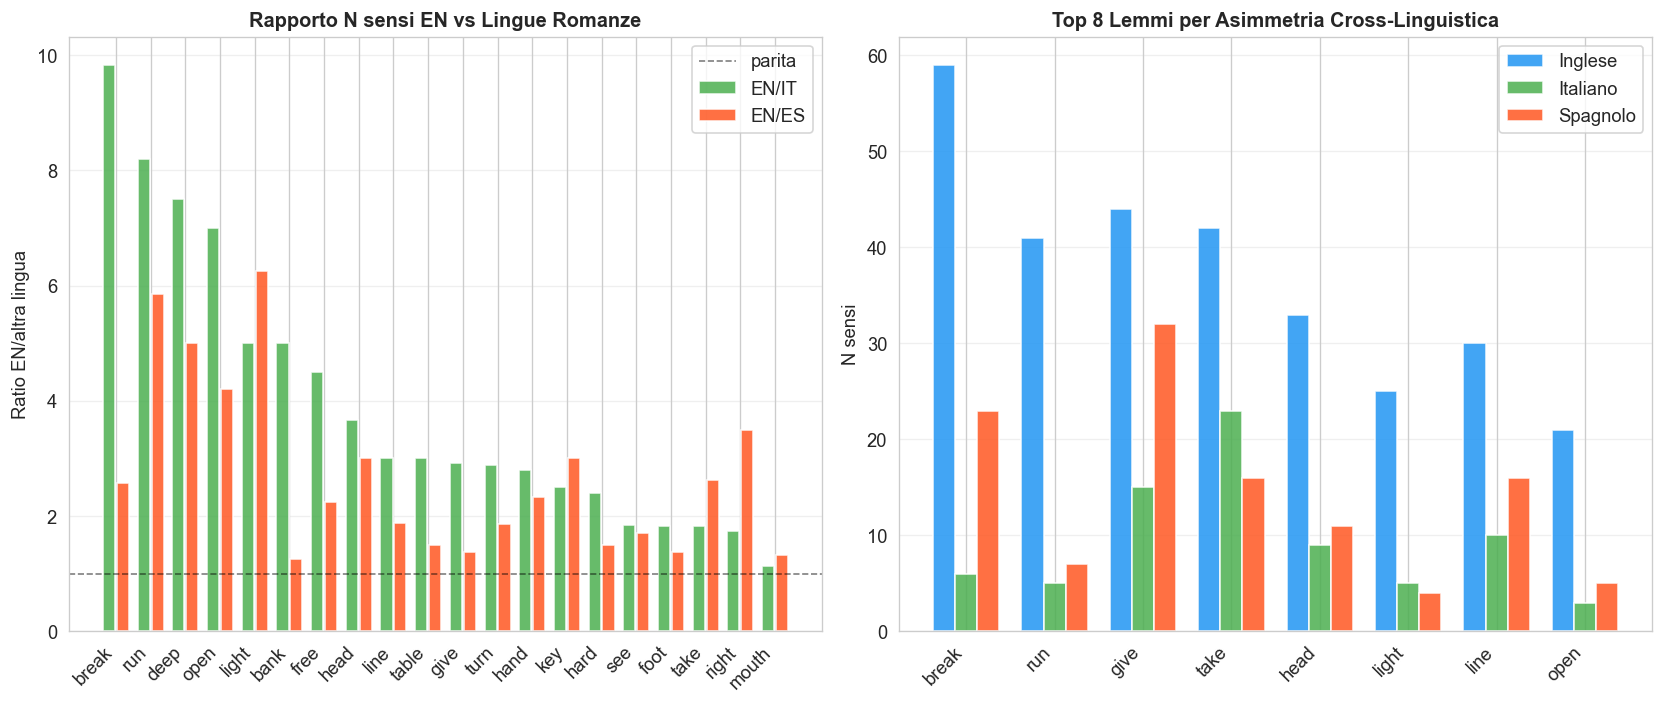
\includegraphics[width=\textwidth]{asimmetrie.png}
  \caption{Sinistra: rapporto EN/IT ed EN/ES per ciascun lemma. Destra: confronto diretto del numero di sensi per i 8 lemmi pi\`u asimmetrici.}
  \label{fig:asimmetrie}
\end{figure}

Il pannello sinistro di Figura~\ref{fig:asimmetrie} mostra che per il lemma \textit{run} il rapporto EN/ES raggiunge $8.14$ (57 sensi inglesi contro 7 spagnoli): un fattore di oltre $8\times$. Il rapporto EN/IT pi\`u alto si osserva per \textit{break} ($12.5\times$). Questi valori estremi confermano quantitativamente l'intuizione qualitativa delle dispense: ``la stessa area semantica pu\`o essere lessicalizzata in modi diversi'' -- in questo caso, l'inglese concentra un numero molto maggiore di accezioni sotto un'unica forma lessicale.

% ============================================================
\section{Discussione}
\label{sec:discussione}
% ============================================================

\subsection{La gerarchia EN $\gg$ ES $>$ IT non \`e (solo) linguistica}

Il risultato pi\`u robusto -- la media di 31.7 sensi in inglese contro 13.2 in spagnolo e 7.95 in italiano -- deve essere interpretato con cautela. Princeton WordNet (la base della parte inglese di OMW) \`e una risorsa costruita e raffinata per oltre 30 anni da linguisti computazionali, con una granularit\`a dei sensi spesso molto fine (lo stesso problema della granularit\`a discusso nelle dispense, Cap.~1: WordNet distingue sensi che un parlante non percepirebbe come distinti). Le estensioni multilingue di OMW per italiano e spagnolo sono invece mappature pi\`u recenti e meno esaustive. Una parte della differenza osservata \`e quindi plausibilmente dovuta a \textbf{differenze nella copertura e nella granularit\`a delle risorse}, non solo a una reale differenza di polisemia tra le lingue -- una limitazione importante da segnalare, in linea con l'invito delle dispense a non considerare il numero di sensi nel dizionario come misura definitiva (Cap.~4: ``una parola pu\`o avere molti sensi nel dizionario, ma usarne abitualmente solo pochi'').

\subsection{Il caso \textit{bank}: asimmetria semantica, non solo quantitativa}

Il lemma \textit{bank} (18 sensi EN, 2 IT, 8 ES) \`e istruttivo non solo per il numero ma per la \textbf{struttura} dei sensi. In italiano, ``banca'' (2 sensi) copre quasi esclusivamente l'istituto finanziario: il senso ``riva del fiume'' \`e lessicalizzato in una parola completamente diversa (\textit{riva}), non tracciata in questo studio per il lemma \textit{bank}. In spagnolo, invece, ``banco'' (8 sensi) \`e semanticamente pi\`u carico: copre l'istituto finanziario, ma anche il mobile (panca/banco di scuola) e il banco di sabbia/pesci -- un comportamento pi\`u vicino a quello inglese, dove \textit{bank} include gi\`a il significato geografico oltre a quello finanziario. Questo \`e un esempio concreto di \textbf{asimmetria cross-linguistica nella lessicalizzazione}: la stessa area concettuale viene divisa diversamente tra le tre lingue, esattamente il fenomeno teorizzato nelle dispense con l'esempio italiano ``tempo'' (atmosferico + cronologico) vs.\ l'inglese (\textit{weather}/\textit{time} separati).

\subsection{\textit{run} e \textit{break}: i casi di massima asimmetria}

I due lemmi con asimmetria pi\`u estrema sono entrambi verbi: \textit{run} (52) e \textit{break} (69). Questo \`e in linea con l'osservazione delle dispense secondo cui i verbi tendono a presentare ``polisemia molto elevata'' in inglese (lo stesso esempio di \textit{run} \`e citato esplicitamente nel Cap.~4 delle dispense). Il verbo inglese \textit{run} si estende infatti a domini semantici molto eterogenei -- corsa fisica, gestione (\textit{run a business}), funzionamento di macchine (\textit{the engine runs}), candidatura politica (\textit{run for office}), liquidi che scorrono -- ciascuno dei quali in italiano e spagnolo \`e tipicamente lessicalizzato con un verbo distinto (\textit{correre}, \textit{gestire}, \textit{funzionare}, \textit{candidarsi}, \textit{scorrere}), motivando direttamente il basso numero di sensi rilevato per ``correre''/``correr'' (5 e 7 rispettivamente), che in OMW intercetta solo l'accezione di movimento fisico.

\subsection{I lemmi pi\`u stabili cross-linguisticamente}

All'estremo opposto, \textit{mouth} (asimmetria 5) e \textit{table} (asimmetria 6) mostrano comportamento pi\`u omogeneo tra le lingue. Si tratta di due sostantivi concreti con un referente fisico ben definito (la bocca, il tavolo): coerentemente con quanto discusso a proposito dei concetti \textbf{Concrete Generic/Specific} nei laboratori 1-2, il vincolo del referente fisico limita anche la variabilit\`a del numero di estensioni di significato disponibili, in tutte e tre le lingue.

\subsection{Implicazioni per il NLP multilingue}

I risultati confermano in modo quantitativo le implicazioni discusse nelle dispense (Cap.~4.5.3): un sistema di \textbf{machine translation} o di \textbf{cross-lingual transfer} che assuma una corrispondenza 1:1 tra i sensi di un lemma inglese e quelli del corrispettivo italiano o spagnolo commetterebbe un errore sistematico, specialmente per verbi ad alta polisemia come \textit{run} o \textit{break}: un modello addestrato sulla granularit\`a fine di WordNet inglese, se applicato senza adattamento a un dominio italiano o spagnolo, tender\`a a generare ambiguit\`a spurie o a fallire nel mappare correttamente le accezioni.

% ============================================================
\section{Conclusioni}
% ============================================================

Il laboratorio ha verificato empiricamente, su 20 lemmi e tre lingue, la tesi delle dispense secondo cui \textbf{non esiste una polisemia universale}: il numero di sensi disponibili per lo stesso lemma varia sistematicamente tra inglese, italiano e spagnolo (rispettivamente 31.7, 7.95 e 13.15 sensi medi), con asimmetrie individuali fino a $12.5\times$ (\textit{break}, EN/IT) e $8.14\times$ (\textit{run}, EN/ES).

I risultati principali sono:

\begin{enumerate}
  \item \textbf{Gerarchia sistematica EN $\gg$ ES $>$ IT}, confermata sia nell'aggregato sia all'interno di ogni categoria grammaticale (sostantivi, verbi, aggettivi) -- ma da interpretare cum grano salis, essendo in parte attribuibile a differenze di copertura/granularit\`a tra le risorse lessicali, non solo a una reale differenza di polisemia.
  \item \textbf{I verbi mostrano l'asimmetria pi\`u marcata} (\textit{break}, \textit{run}), coerentemente con la tendenza dei verbi inglesi a un'estensione semantica molto ampia rispetto alle lingue romanze.
  \item \textbf{I sostantivi concreti con referente fisico stabile} (\textit{mouth}, \textit{table}, \textit{foot}) mostrano la minore asimmetria cross-linguistica, suggerendo che il vincolo referenziale limiti la variabilit\`a anche a livello multilingue.
  \item \textbf{L'asimmetria non \`e solo quantitativa ma strutturale}: il caso \textit{bank}/\textit{banca}/\textit{banco} mostra come la stessa area concettuale possa essere ripartita in modo diverso tra parole distinte (italiano) o concentrata in un'unica forma pi\`u carica semanticamente (spagnolo, pi\`u vicino all'inglese).
\end{enumerate}

Il limite principale dello studio \`e l'assunzione di \textbf{distribuzione uniforme dei sensi} per tutte le lingue, dovuta all'assenza di dati di frequenza d'uso in OMW per italiano e spagnolo (a differenza dell'inglese, dove tali dati esistono via SemCor). Un'estensione naturale del lavoro sarebbe integrare stime di frequenza per le lingue romanze (es.\ da corpora annotati o da conteggi su corpora di testo generici), permettendo di calcolare un'entropia realistica e non semplicemente $\log_2 n$, e di distinguere lemmi con \emph{molti sensi ma fortemente dominati da un uso comune} da lemmi con sensi realmente equiprobabili -- la distinzione esplicitamente evidenziata come cruciale nelle dispense (Cap.~4.7, ``distribuzione sbilanciata della complessit\`a'').

\end{document}
